
\documentclass[twoside,onecolumn]{article}

\usepackage{blindtext} % Package to generate dummy text throughout this template 

%\usepackage[sc]{mathpazo} % Use the Palatino font
\usepackage[T1]{fontenc} % Use 8-bit encoding that has 256 glyphs
\linespread{1.05} % Line spacing - Palatino needs more space between lines
\usepackage{microtype} % Slightly tweak font spacing for aesthetics
\usepackage{float}
 \usepackage{amsmath}
 \usepackage{booktabs}
 \usepackage{amssymb}
 \usepackage{amsthm}
 \usepackage{tabularx} %tabelle
 \usepackage{tikz} %circuiti
 \usepackage{enumerate}
 \usepackage{pgfplots}
 \usepackage{subcaption}
\usepackage[toc,page]{appendix}
 \usepackage[export]{adjustbox}
 \usepackage{caption}
 \usepackage{subfig}
 \usepackage{sidecap}
 \usepackage{algorithm}

 \usepackage{graphicx}
 \theoremstyle{definition}
  \usepackage{multicol}
  \usetikzlibrary{arrows}
  \usepackage{algpseudocode}
\usepackage{multirow}
\usepackage{mathtools}
\usepackage{array, caption}
\usepackage{graphicx}
\usepackage{makecell}
  
\usepackage[english]{babel} % Language hyphenation and typographical rules

\usepackage[hmarginratio=1:1,top=32mm,columnsep=20pt]{geometry} % Document margins
\usepackage[hang, small,labelfont=bf,up,textfont=it,up]{caption} % Custom captions under/above floats in tables or figures
\usepackage{booktabs} % Horizontal rules in tables

\usepackage{lettrine} % The lettrine is the first enlarged letter at the beginning of the text

\usepackage{enumitem} % Customized lists
\setlist[itemize]{noitemsep} % Make itemize lists more compact

\usepackage{titlesec} % Allows customization of titles
\titleformat{\section}[block]{\large\scshape\centering}{\thesection.}{1em}{} % Change the look of the section titles
\titleformat{\subsection}[block]{\large}{\thesubsection.}{1em}{} % Change the look of the section titles

\usepackage{hyperref} % For hyperlinks in the PDF

\title{Lab 3: Edge, lines and circles detection } % Article title
\author{Nicole Zattarin}
\date{} 
\begin{document}

% Print the title
\maketitle

\begin{abstract}
ciao belli
\end{abstract}

\section{Setup and parameters tuning}
\begin{figure} \centering
\begin{subfigure}{0.5\textwidth}
  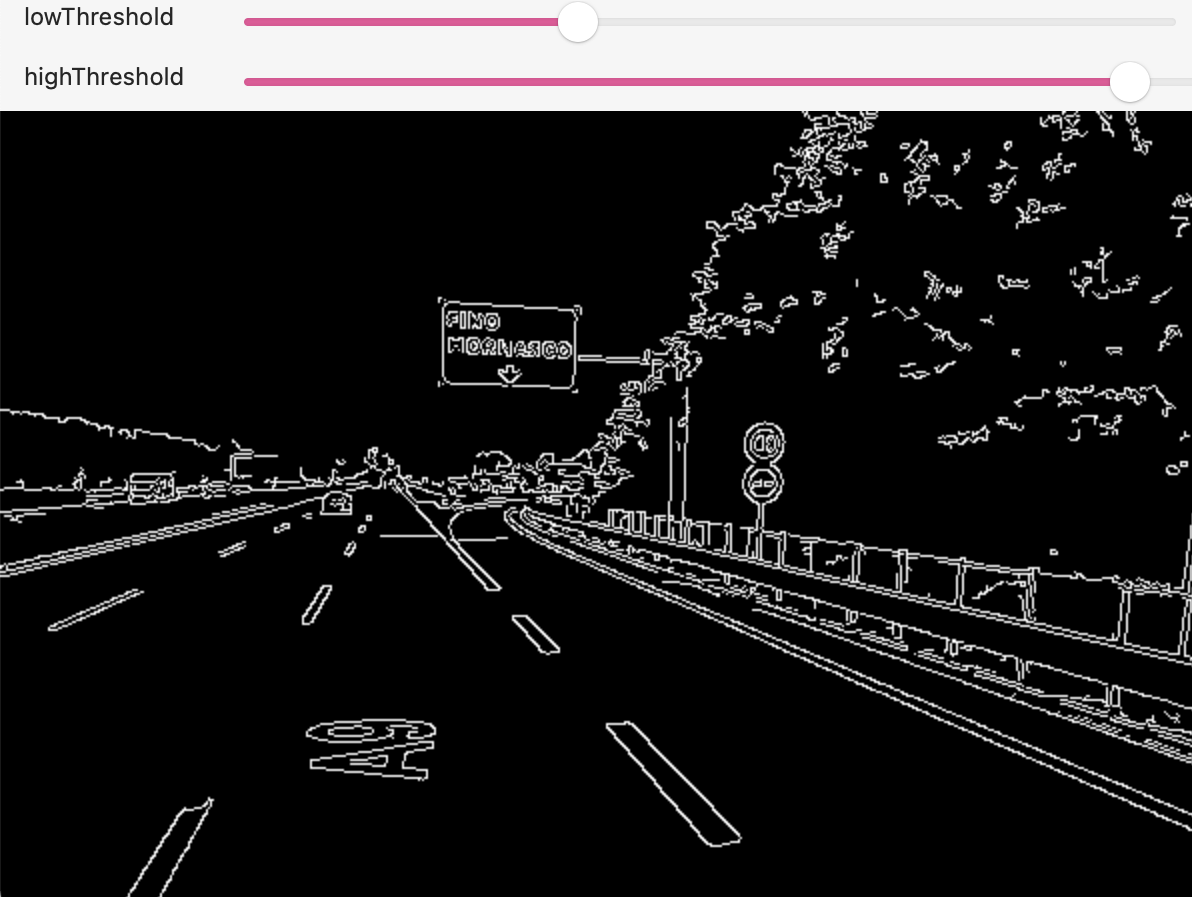
\includegraphics[width=\textwidth]{../results/tuningEdge.png}
\caption{ }\label{fig:tuningedge}
\end{subfigure} \quad
\begin{subfigure}{0.46\textwidth}
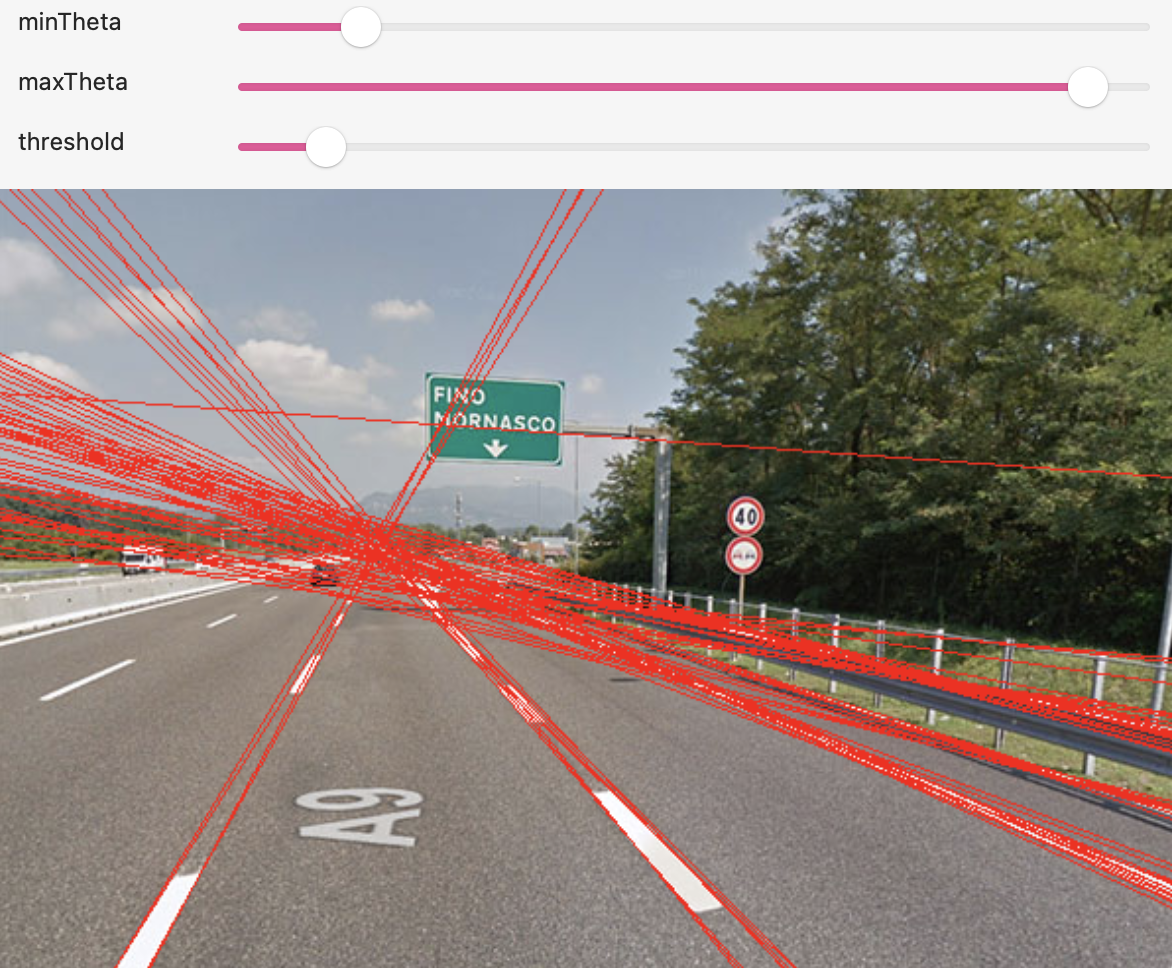
\includegraphics[width=\textwidth]{../results/tuningLines.png}
\caption{}\label{fig:tuningline}
\end{subfigure}\caption{}\label{fig:tuning}
\end{figure}


\section{Results}
% ROAD2

\begin{table}\centering
\begin{tabular}[b]{ |c|c|c| }
\hline
\multirow{8}{*}[6.5ex]{\rotatebox{90}{Canny}} 
 & apertureSize & 3 \\
 & threshold1  & 350 \\
 & threshold2 & 850\\  \hline
\end{tabular}
\hskip
\begin{tabular}[b]{ |c|c|c| }
\hline
\multirow{8}{*}[4ex]{\rotatebox{90}{HoughLines}} 
& rho &  1 \\
 & theta & 0.05 \\
 &threshold& 130\\
  & min theta  & 0\\ 
 & max theta  & CV PI\\ \hline
\end{tabular}
\hskip
\begin{tabular}[b]{ |c|c|c| }
\hline
\multirow{8}{*}[3ex]{\rotatebox{90}{HoughCircles}} 
& dp & 1 \\
 & minDist & 1\\
 & param1& 100 \\
  & param2& 25 \\ 
    & minRadius& 0 \\ 
 & maxRadius & 10 \\ \hline
\end{tabular}
\caption{ROAD2} \label{tab:r2}
\end{table}


\begin{figure} \centering
\begin{subfigure}{0.8\textwidth}
  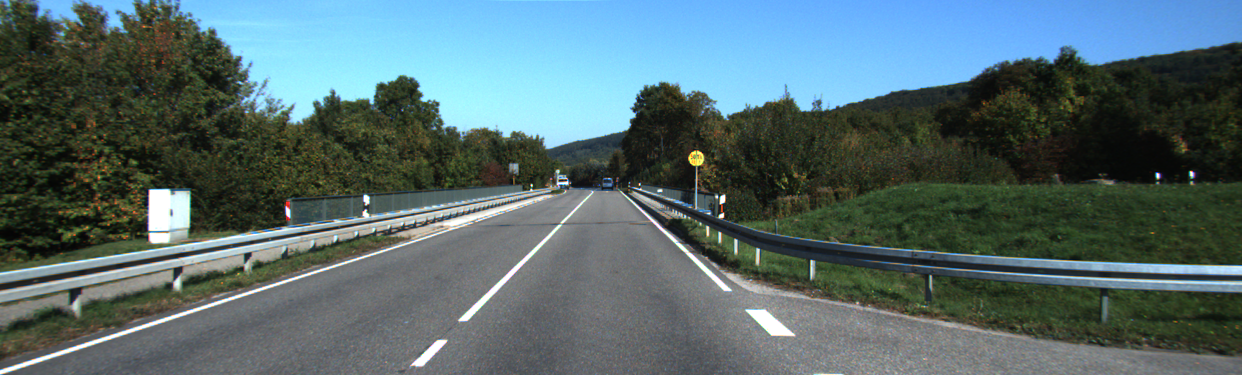
\includegraphics[width=\textwidth]{../images/road2.png}
\caption{ }\label{fig:r2fig}
\end{subfigure} \\
\begin{subfigure}{0.8\textwidth}
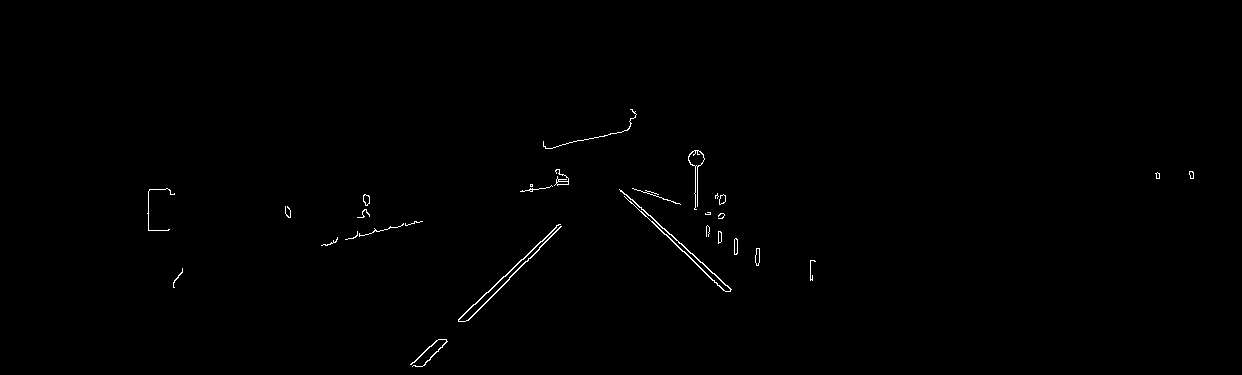
\includegraphics[width=\textwidth]{../results/edgeMap_road2.png}
\caption{}\label{fig:road2edges}
\end{subfigure}
  \begin{subfigure}{0.8\textwidth}
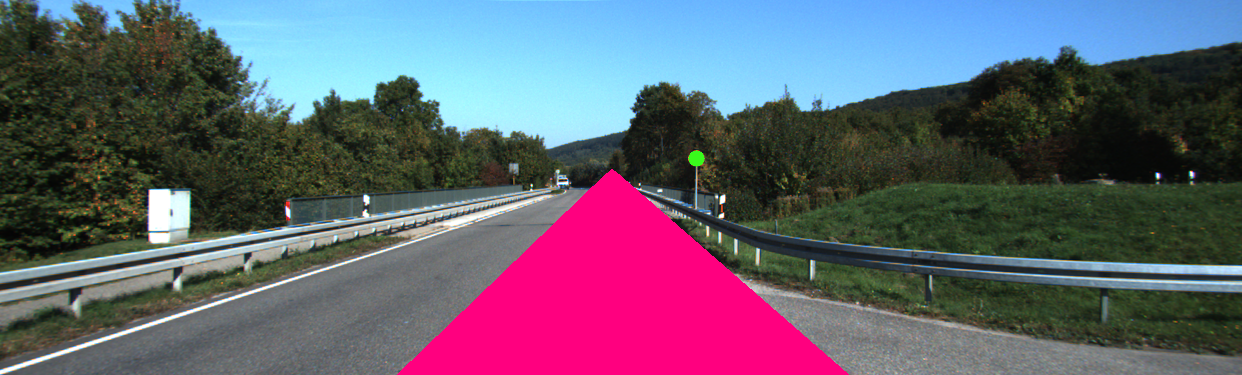
\includegraphics[width=\textwidth]{../results/Circles_road2.png}
\caption{}\label{fig:road2circles}
\end{subfigure}\caption{}\label{fig:road2}
\end{figure}

%ROAD3
\begin{table}\centering
  \begin{tabular}[b]{ |c|c|c| }
  \hline
  \multirow{8}{*}[6.5ex]{\rotatebox{90}{Canny}} 
   & apertureSize & 3 \\
   & threshold1  & 270 \\
   & threshold2 & 400\\  \hline
  \end{tabular}
  \hskip
  \begin{tabular}[b]{ |c|c|c| }
  \hline
  \multirow{8}{*}[4ex]{\rotatebox{90}{HoughLines}} 
  & rho &  1 \\
   & theta & 0.05 \\
   &threshold& 160\\
    & min theta  & 0\\ 
   & max theta  & 3\\ \hline
  \end{tabular}
  \hskip
  \begin{tabular}[b]{ |c|c|c| }
  \hline
  \multirow{8}{*}[3ex]{\rotatebox{90}{HoughCircles}} 
  & dp & 1 \\
   & minDist & 1\\
   & param1& 353 \\
    & param2& 31 \\ 
      & minRadius& 0 \\ 
   & maxRadius & 32 \\ \hline
  \end{tabular}
  \caption{ROAD3} \label{tab:r2}
  \end{table}

  
\begin{figure} \centering
\begin{subfigure}{0.45\textwidth}
  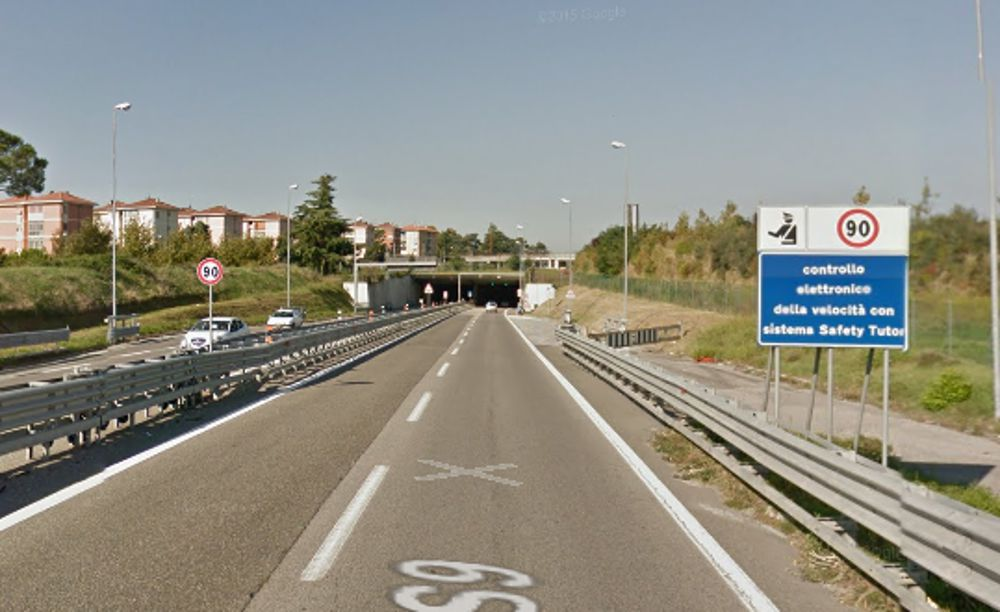
\includegraphics[width=\textwidth]{../images/road3.jpg}
\caption{ }\label{fig:r3fig}
\end{subfigure} \quad
\begin{subfigure}{0.45\textwidth}
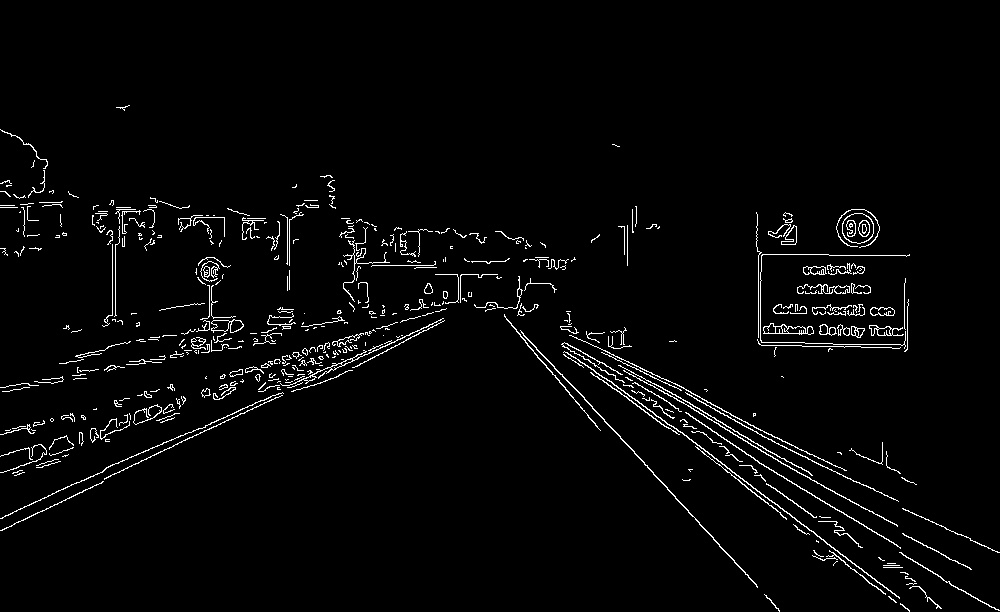
\includegraphics[width=\textwidth]{../results/edgeMap_road3.jpg}
\caption{}\label{fig:road3edges}
\end{subfigure}\\
  \begin{subfigure}{0.6\textwidth}
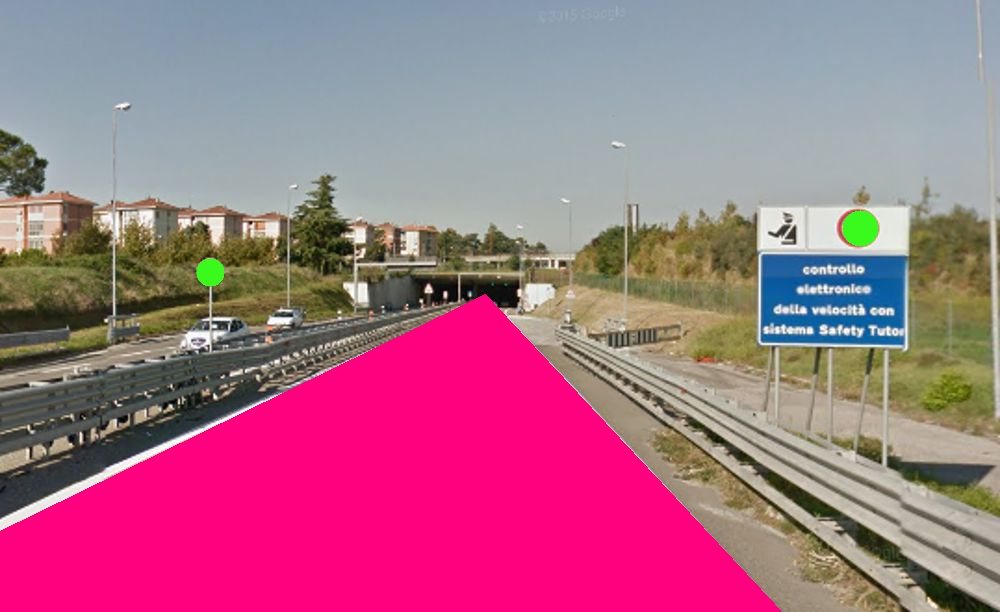
\includegraphics[width=\textwidth]{../results/Circles_road3.jpg}
\caption{}\label{fig:road3circles}
\end{subfigure}\caption{}\label{fig:road3}
\end{figure}



%ROAD4
\begin{table}\centering
  \begin{tabular}[b]{ |c|c|c| }
  \hline
  \multirow{8}{*}[6.5ex]{\rotatebox{90}{Canny}} 
   & apertureSize & 3 \\
   & threshold1  & 450 \\
   & threshold2 & 730\\  \hline
  \end{tabular}
  \hskip
  \begin{tabular}[b]{ |c|c|c| }
  \hline
  \multirow{8}{*}[4ex]{\rotatebox{90}{HoughLines}} 
  & rho &  1 \\
   & theta & 0.05 \\
   &threshold& 62\\
    & min theta  & 1\\ 
   & max theta  & 3\\ \hline
  \end{tabular}
  \hskip
  \begin{tabular}[b]{ |c|c|c| }
  \hline
  \multirow{8}{*}[3ex]{\rotatebox{90}{HoughCircles}} 
  & dp & 1 \\
   & minDist & 1\\
   & param1& 67 \\
    & param2& 31 \\ 
      & minRadius& 0 \\ 
   & maxRadius & 14 \\ \hline
  \end{tabular}
  \caption{ROAD4} \label{tab:r2}
  \end{table}


\begin{figure} \centering
\begin{subfigure}{0.45\textwidth}
  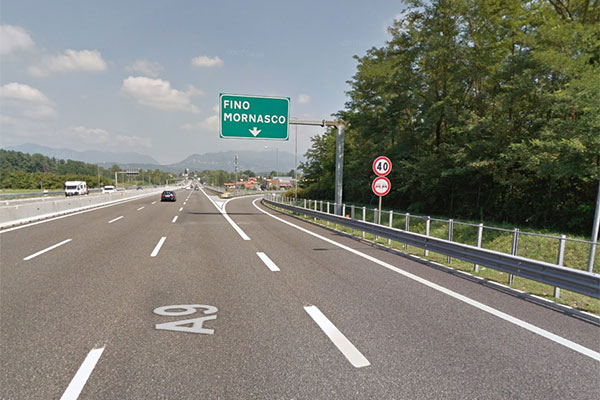
\includegraphics[width=\textwidth]{../images/road4.jpg}
\caption{ }\label{fig:r4fig}
\end{subfigure} \quad
\begin{subfigure}{0.45\textwidth}
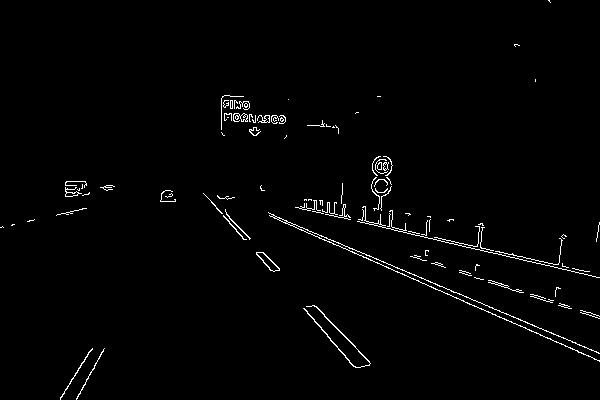
\includegraphics[width=\textwidth]{../results/edgeMap_road4.jpg}
\caption{}\label{fig:road4edges}
\end{subfigure}\\
  \begin{subfigure}{0.6\textwidth}
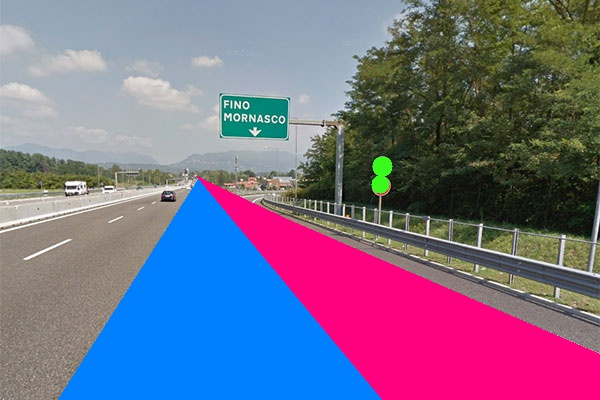
\includegraphics[width=\textwidth]{../results/Circles_road4.jpg}
\caption{}\label{fig:road4circles}
\end{subfigure}\caption{}\label{fig:road4}
\end{figure}



\end{document}

